% Chapter 3

\chapter{Extrapolating average accuracy} % Main chapter title

\newcommand{\skone}{\mathcal{S}_{k_1}}
\newcommand{\sktwo}{\mathcal{S}_{k_2}}


\label{Chapter3} % For referencing the chapter elsewhere, use \ref{Chapter1} 

\section{Introduction}

In this chapter, we address the question of how to estimate the
$k$-class average accuracy, $\text{AGA}_{k, r}$, based on data from a
problem $P_1$ with $k_1 < k$ classes, and $r = r_1$-repeat training
data.  We continue with the framework introduced in Chapter 2,
including the definition of the average risk and the marginal property
of classifiers.

We begin by continuing to analyze the average accuracy $\text{AGA}_{k,
  r}$, which results in an explicit formula for the average accuracy.
The formula reveals that all of the information needed to compute the
average accuracy is contained in a one-dimensional function $\bar{D}(u)$,
and therefore that estimation of the average accuracy can be accomplished
via estimation of the unknown function $\bar{D}(u)$.  This allows the
development of a class of unbiased estimators of $\bar{D}(u)$,
presented in section \ref{sec:extrapolation_estimation} given the
assumption of a known parametric form for $\bar{D}(u)$.  We analyze
the performance of the estimator in both the well-specified and
misspecified case.  We demonstrate our method to a face-recognition
example in section \ref{sec:extrapolation_example}.  Additionally, in
Chapter 5 %% cite the specific section later we will see the
comparison of the estimator to an alternative, information-theory
based estimator in simulated and real-data examples.

\section{Analysis of average risk}

The result of our analysis is to expose the average accuracy
$\text{AGA}_{k, r}$ as the weighted average of a function
$\bar{D}(u)$, where $\bar{D}(u)$ is independent of $k$, and where $k$
only changes the weighting.  The result is stated as follows.

\begin{theorem}\label{theorem:avrisk_identity}
Suppose $\pi$, $\{F_y\}_{y \in \mathcal{Y}}$ and marginal classifier
$\mathcal{F}$ satisfy the tie-breaking condition.  Then, under the
definitions \eqref{eq:U_function}, \eqref{eq:Kfunc},
and \eqref{eq:Kbar}, we have
\begin{equation}\label{eq:avrisk_identity}
\text{AGA}_{k, r} = 1 - (k-1) \int \bar{D}(u) u^{k-2} du.
\end{equation}
\end{theorem}

The tie-breaking condition referred in the theorem is defined as follows.
\begin{itemize}
\item 
\emph{Tie-breaking condition}: for all $x \in \mathcal{X}$,
$\mathcal{M}(\hat{F}_Y)(x) = \mathcal{M}(\hat{F}_{Y'})(x)$
with zero probability for $Y, Y'$ independently drawn from $\pi$.
\end{itemize}
The tie-breaking condition is a technical assumption which allows us
to neglect the specification of a tie-breaking rule in the case that
margins are tied.  In practice, one can simply break ties randomly,
which is mathematically equivalent to adding a small amount of random
noise $\epsilon$ to the function $\mathcal{M}$.

\iffalse

Let us revisit the definition of the average risk, under a general
cost function $C$.  The $k$-class, $r$-repeat \emph{average risk} of a
marginal classifier $\mathcal{M}$ is defined as
\begin{align*}
\text{AvRisk}_{k,r_1}(\mathcal{M}) &= \E[\text{Risk}_{\mathcal{S}}(\mathcal{M})|Y^{(1)}, \hdots, Y^{(k)} \sim \pi]
\\&= \frac{1}{k} \sum_{i=1}^k \int
I(\mathcal{M}(\hat{F}_{y^{(i)}})(x) \neq \max_j
\mathcal{M}(\hat{F}_{y^{(j)}})) dF_{y^{(i)}}(x) \prod_{\ell=1}^k
d\Pi_{y^{(\ell)}, r_1}(\hat{F}_{y^{(\ell)}}) d\pi(y^{(\ell)}).
\end{align*}
The definition of average risk is illustrated in Figure \ref{fig:average_risk2}.

\begin{figure}[h]
\centering
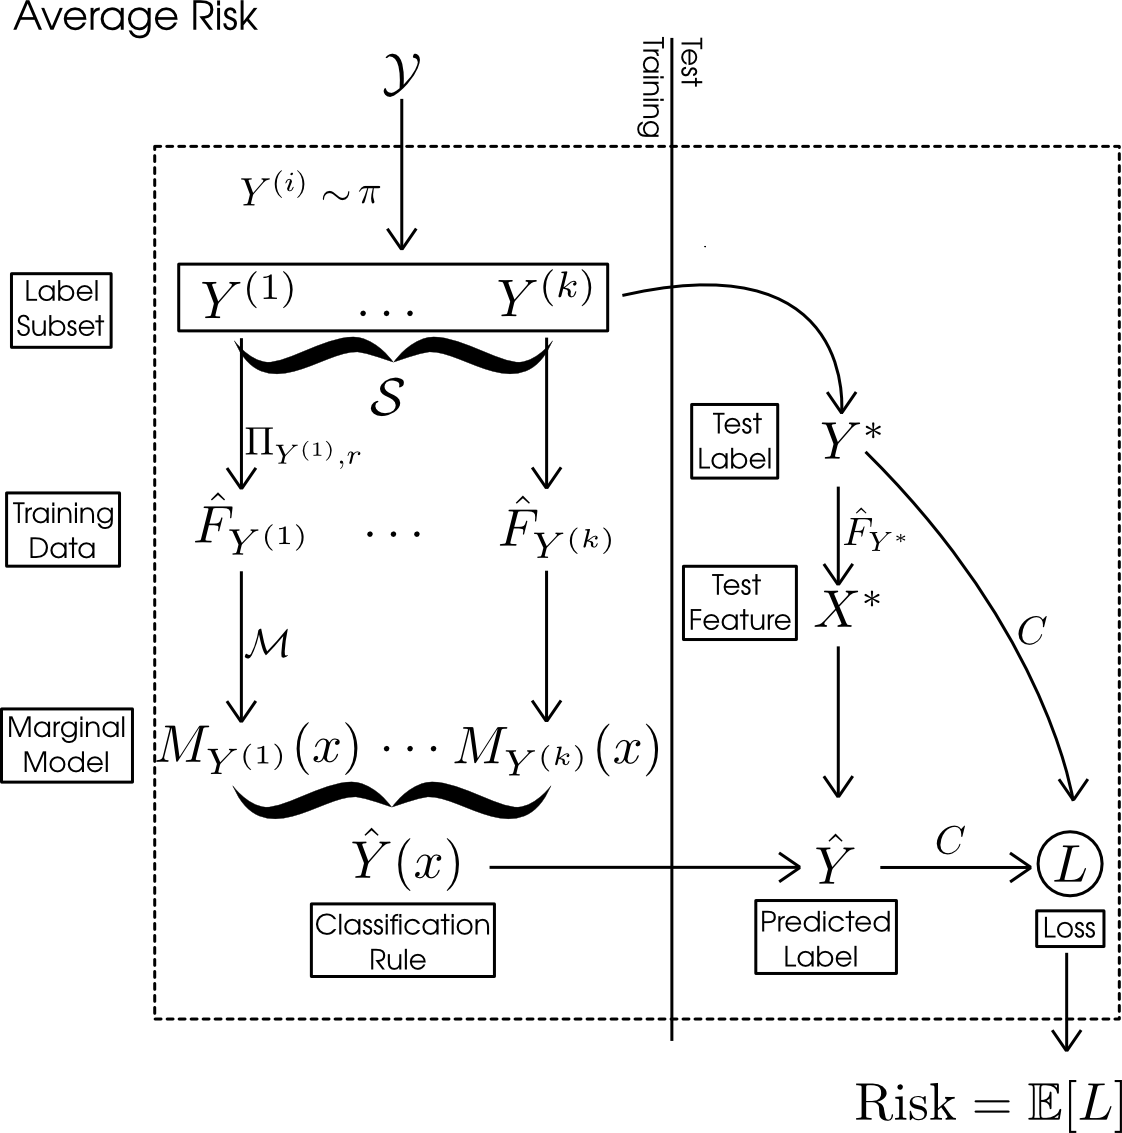
\includegraphics[scale = 0.3]{../extrapolation_figures/average_risk.png}
\caption{Average risk}\label{fig:average_risk2}
\end{figure}

\fi

As we can see from Figure \ref{fig:average_risk}, the average accuracy is
obtained by averaging over four randomizations:
\begin{enumerate}
\item[A1.] Drawing the label subset $\mathcal{S}$.
\item[A2.] Drawing the training dataset.
\item[A3.] Drawing $Y^*$ uniformly at random from $\mathcal{S}$.
\item[A4.] Drawing $X^*$ from $F_{X^*}$.
\end{enumerate}


Our strategy is to analyze the average accuracy by
means of \emph{conditioning on} the true label and its training
sample, $(y^*, \hat{F}_{y^*})$, and the test feature $x^*$
while \emph{averaging} over all the other random variables.  Define
the \emph{conditional accuracy} $\text{CondAcc}_k((y^*, \hat{F}_{y^*}), x^*)$ as
\[
\text{CondAcc}_k((y^*, \hat{F}_{y^*}), x^*) = \Pr[\argmax_{y \in \mathcal{S}} \mathcal{M}(\{\hat{F}_y\})(X^*) = Y^* |Y^*=y^*, X^* = x^*, \hat{F}_{Y^*} = \hat{F}_{y^*}].
\]
Figure \ref{fig:conditional_risk} illustrates the variables which are
fixed under conditioning and the variables which are randomized.
Compare to figure \ref{fig:average_risk}.

Without loss of generality, we can write the label subset $\mathcal{S}
= \{Y^*, Y^{(1)},\hdots, Y^{(k-1)}\}$.  Note that due to independence,
$Y^{(1)},\hdots, Y^{(k-1)}$ are still i.i.d. from $\pi$ even
conditioning on $Y^* = y^*.$ Therefore, the conditional risk can be
obtained via the following alternative order of randomizations:
\begin{enumerate}
\item[C0.] 
Fix $y^*, \hat{F}_y^*,$ and $x^*$.  Note that $M_{y^*}(x^*)
= \mathcal{M}(\hat{F}_{y^*})(x^*)$ is also fixed.
\item[C1.]
Draw the \emph{incorrect labels} $Y^{(1)},\hdots, Y^{(k)}$ i.i.d. from
$\pi$.  (Note that $Y^{(i)} \neq y^*$ with probability 1 due to the
continuity assumptions on $\mathcal{Y}$ and $\pi$.)
\item[C2.]
Draw the training samples for the incorrect labels
$\hat{F}_{Y^{(1)}},\hdots, \hat{F}_{Y^{(k-1)}}$.  This determines
\[
\hat{Y} = \argmax_{y \in \mathcal{S}} M_y(x^*)
\]
and hence, whether or not the classification is correct for $(x^*, y^*)$
\end{enumerate}
Compared to four randomization steps for the average risk, we have
essentially conditioned on steps A3 and A4 and randomized over steps
A1 and A2.

\begin{figure}[h]
\centering
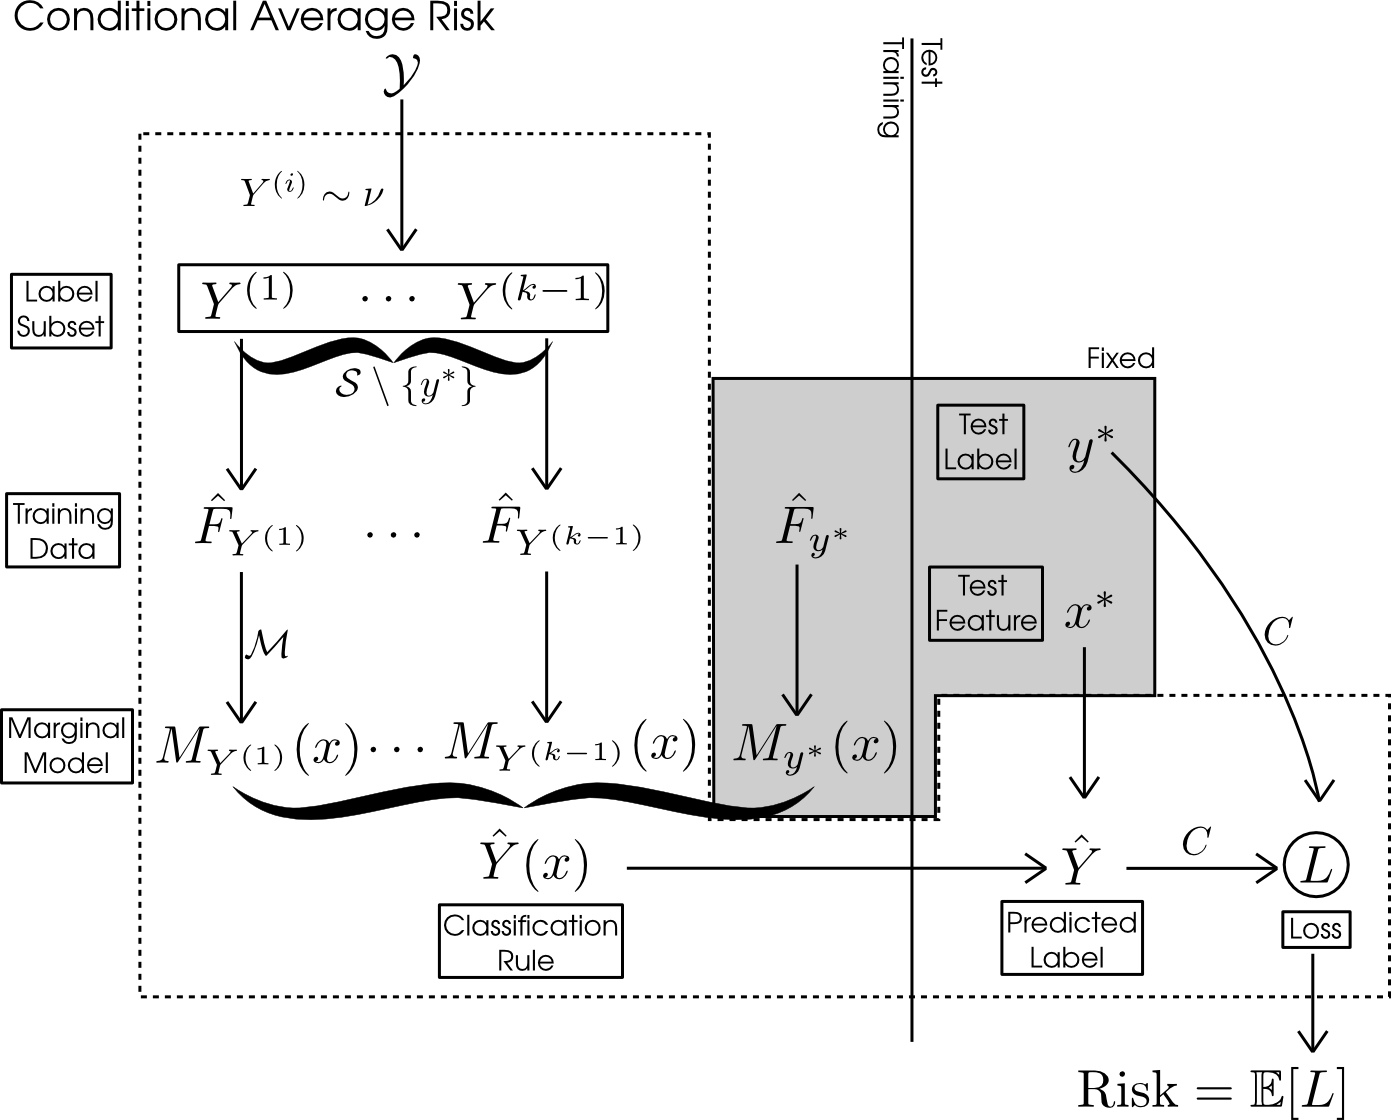
\includegraphics[scale = 0.3]{../extrapolation_figures/conditional_risk.png}
\caption{Conditional accuracy [note: figure needs to be fixed!]}\label{fig:conditional_risk}
\end{figure}

Now, in order to analyze the $k$-class behavior of the conditional
accuracy, we begin by considering the \emph{two-class} situation.

In the two-class situation, we have a true label $y^*$, a training
sample $\hat{F}_{y^*}$, and one incorrect label, $Y$.  Define the
\emph{U-function} $U_{x^*}(y^*, \hat{F}_{y^*})$ as the conditional
accuracy (the probability of correct classification) in the two-class
case.  The classification is correct if the margin $M_{y^*}(x^*)$ is
greater than the margin $M_Y(x^*)$, and incorrect otherwise.  Since we
are fixing $x^*$ and $(y^*, \hat{F}_{y^*})$, the probability of
correct classification is obtained by taking an expectation:
\begin{align}\label{eq:U_function}
U_{x^*}(y^*, \hat{F}_{y^*}) &= \Pr[M_{y^*}(x^*) > \mathcal{M}(\hat{F}_Y)(x^*)]
\\&= \int_{\mathcal{Y}} 
I\{
M_{y^*}(x^*) > \mathcal{M}(\hat{F}_{y})(x)
\}
d\Pi_{y, r}(\hat{F}_y)
d\pi(y).
\end{align}
See also figure \ref{fig:U_function} for an graphical illustration of
the definition.

\begin{figure}[h]
\centering
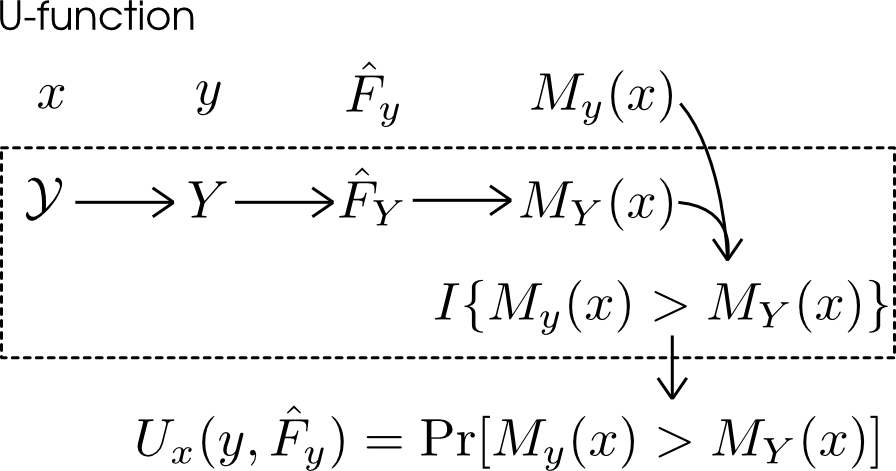
\includegraphics[scale = 0.4]{../extrapolation_figures/U_function.png}
\caption{U-functions}\label{fig:U_function}
\end{figure}

An important property of the U-function, and the basis for its name,
is that the random variable $U_x(Y, \hat{F}_Y)$ for $Y \sim \pi$ and
$\hat{F}_Y \sim \Pi_{Y, r}$ is uniformly distributed for all
$x \in \mathcal{X}$.  This is proved in Lemma \ref{lemma:U_function}
in Appendix C.

Now, we will see how the U-function allows us to understand the
$k$-class case.  Suppose we have true label $y^*$ and incorrect labels
$Y^{(1)},\hdots, Y^{(k-1)}$.  Note that the U-function
$U_{x^*}(y, \hat{F}_y)$ is monotonic in $M_y(x^*)$.  Therefore,
\[
\hat{Y} = \argmax_{y \in \mathcal{S}} M_y(x^*) = \argmax_{y \in \mathcal{S}} U_{x^*}(y, \hat{F}_y).
\]
Therefore, we have a correct classification if and only if the U-function value for the correct label
is greater than the maximum U-function values for the incorrect labels:
\[
\Pr[\hat{Y} = y^*] = \Pr[U_{x^*}(y^*, \hat{F}_{y^*}) > \max_{i=1}^{k-1} U_{x^*}(Y^{(i)}, \hat{F}_{Y^{(i)}})] =  \Pr[u^* > U_{max}].
\]
where $u^* = U_{x^*}(y^*, \hat{F}_{y^*})$ and $U_{max, k-1}
= \max_{i=1}^{k-1} U_{x^*}(Y^{(i)}, \hat{F}_{Y^{(i)}})$.  But now,
observe that we know the distribution of $U_{max, k-1}$!  Since
$U_{x^*}(Y^{(i)}, \hat{F}_{Y^{(i)}})$ are i.i.d. uniform, we know that
\begin{equation}\label{eq:umax_beta}
U_{max, k-1} \sim \text{Beta}(k-1, 1). 
\end{equation}

Therefore, in the general case, the conditional accuracy is
\[
\text{CondAcc}_k((y^*, \hat{F}_{y^*}), x^*) = \Pr[U_{max} > u^*] = 1 - \int_{u^*}^1 (k-1) u^{k-2} du.
\]
Now the average accuracy can be obtained by integrating over the
distribution of $U^* = U_{x^*}(y^*, \hat{F}_{y^*})$, which we state in
the following proof of theorem \ref{theorem:avrisk_identity}.

\noindent\textbf{Proof of Theorem \ref{theorem:avrisk_identity}}.
We have
\begin{align*}
\text{AGA}_{k,r} &= \E[ 1 - \int_{U^*}^1 (k-1) u^{k-2} du] 
\\&= 1 - \E[\int_0^1 I\{u \geq U^*\} (k-1) u^{k-2} du ]
\\&= (k-1) \int_0^1 \Pr[U^* \leq u] u^{k-2} du.
\end{align*}
Or equivalently,
\[
\text{AGA}_{k, r}((y^*, \hat{F}_{y^*}), x^*) = 1 - (k-1) \int \bar{D}(u) u^{k-2} du.
\]
where $\bar{D}(u)$ denotes the cumulative distribution function of $U^*$ on $[0,1]$:
\[
\bar{D}(u) = \Pr[U_{x^*}(y^*, \hat{F}_{y^*}) \leq u].
\]
We have expressed the average risk expressed as a weighted integral of
a certain function $\bar{D}(u)$ defined on $u \in [0,1]$.  We have
clearly isolated the part of the average risk which is independent of
$k$--the univariate function $\bar{D}(u)$, and the part which is
dependent on $k$--which is the density of $U_{max}$.

In section \ref{sec:extrapolation_estimation}, we will develop
estimators of $\bar{D}(u)$ in order to estimate the $k$-class average
risk.

Having this theoretical result allows us to understand how the
expected $k$-class risk scales with $k$ in problems where all the
relevant densities are known.  However, applying this result in
practice to estimate $\text{Average Risk}_k$ requires some means of
estimating the unknown function $\bar{D}$--which we discuss in the
following.

\section{Estimation}\label{sec:extrapolation_estimation}

Now we address the problem of estimating $\text{AGA}_{k_2, r_1}$ from
data.  As we have seen from Theorem \ref{theorem:avrisk_identity}, the
$k$-class average accuracy of a marginal classifier $\mathcal{M}$ is a
functional of a object called $\bar{D}(u),$ which depends marginal
model $\mathcal{M}$ of the classifier, the joint distribution of
labels $Y$ and features $X$ when $Y$ is drawn from the sampling
density $\nu$.

Therefore, the strategy we take is to attempt to estimate $\bar{D}$
for then given classification model, and then plug in our estimate of
$\bar{D}$ into the integral \eqref{eq:avrisk_identity} to obtain an
estimate of $\text{AGA}_{k_2, r_{train}}$.

Having decided to estimate $\bar{D}$, there is then the question of
what kind of model we should assume for $\bar{D}$.  In this work, we
assume that some parametric model\footnote{While a
nonparametric approach may be more ideal, we leave this to future work.} is available for $\bar{D}$.

Let us assume the linear model
\begin{equation}\label{eq:linearKu}
\bar{D}(u) = \sum_{\ell = 1}^m \beta_\ell h_\ell(u),
\end{equation}
where $h_\ell(u)$ are known basis functions, and $\beta$ are the model
parameters to be estimated. We can obtain \emph{unbiased} estimation
of $\text{AGA}_{k_2, r_{train}}$ via the unbiased estimates of
$k$-class average risk obtained from \eqref{eq:avtestrisk}.

If we plug in the assumed linear model \eqref{eq:linearKu} into the
identity \eqref{eq:avrisk_identity}, then we get
\begin{align}
1 - \text{AGA}_{k, r_{train}} &= (k-2)\int \bar{D}(u) u^{k-2} du
\\&= (k-2)\int_0^1 \sum_{\ell = 1}^m \beta_\ell h_\ell(u) u^{k-2} du
\\&= \sum_{\ell = 1}^m \beta_\ell H_{\ell,k} \label{eq:avrisk_linear}
\end{align}
where
\begin{equation}
H_{\ell,k} = (k-2) \int_0^1 h_\ell(u) u^{k-2} du.
\end{equation}
The constants $H_{\ell, k}$ are moments of the basis function
$h_\ell$: hence we call this method the \emph{moment method.}  Note
that $H_{\ell, k}$ can be precomputed numerically for any $k \geq 2$.


Now, since the test accuracies $\text{TA}_k$ are unbiased estimates of
$\text{AGA}_{k, r_{train}}$, this implies that the regression
estimate
\[
\hat{\beta} = \argmin_\beta \sum_{k=2}^{k_1} w_k \left( (1 - \text{TA}_k) - \sum_{\ell=1}^m \beta_\ell H_{\ell, k}\right)^2
\]
is unbiased for $\beta$, under any choice of positive weights $w_k$.
The estimate of $\text{AGA}_{k_2,r_1}$ is similarly obtained
from \eqref{eq:avrisk_linear}, via
\begin{equation}\label{eq:avrisk_hat}
\widehat{\text{AGA}_{k_2,r_1}} = \sum_{\ell=1}^m \hat{\beta}_\ell H_{\ell, k_2}.
\end{equation}

\section{Examples}\label{sec:extrapolation_example}

